\chapter{Transformada de Radon y retroproyección filtrada}

En este capítulo se desarrolla el modelo continuo de adquisición tomográfica en geometría paralela y se deriva la fórmula de retroproyección filtrada. Las identidades analíticas se formulan inicialmente para funciones de Schwartz, con las convenciones de Fourier fijadas en el capítulo anterior. El objetivo es obtener, a partir del teorema de corte de Fourier y del cambio a coordenadas polares con radio firmado, la fórmula
\[
f=
\mathcal R^*\mathcal F_t^{-1}
\left[
|\sigma|\,\mathcal F_t(\mathcal Rf)
\right].
\]

\section{Modelo tomográfico y geometría}

En un modelo bidimensional idealizado de tomografía computarizada, una sección del objeto se representa mediante un coeficiente de atenuación
\[
f:\mathbb R^2\to\mathbb R,
\]
no negativo, suficientemente regular y con soporte acotado. Esta función describe la atenuación local que experimenta un haz de rayos X al atravesar el objeto.

La relación física básica entre atenuación y medición se expresa mediante la ley de Beer--Lambert. Si un haz de intensidad inicial $I_0$ recorre una trayectoria $\gamma$ y se mide una intensidad final $I$, entonces, bajo un modelo ideal sin dispersión,
\[
I=I_0\exp\left(-\int_\gamma f(x)\,ds\right).
\]
Por tanto,
\[
-\log\left(\frac{I}{I_0}\right)
=
\int_\gamma f(x)\,ds.
\]
Así, después de normalizar la intensidad y tomar logaritmos, el dato medido es una integral de línea del coeficiente de atenuación. Esta idealización y su conexión con el modelo tomográfico se presentan, por ejemplo, en Kuchment \cite[Sec.~5.3.1, pp.~23--25]{kuchment2014}.

La Figura~\ref{fig:beer-lambert} resume esta etapa física: el detector no mide directamente $f$, sino una intensidad atenuada cuya normalización logarítmica produce una integral sobre la trayectoria del haz.

\begin{figure}[htbp]
\centering
\resizebox{0.86\textwidth}{!}{\shorthandoff{<>}
\begin{tikzpicture}[font=\small]
    \draw[draw=black, fill=gray!15, thick] (0,0) ellipse (1.25 and 0.85);
    \node at (0,0.18) {objeto};
    \node at (0,-0.23) {$f(x)$};

    \draw[fill=black!10, draw=black, thick] (-4,0.55) -- (-3.35,0.9) -- (-3.35,0.2) -- cycle;
    \draw[fill=black!35, draw=black] (-4.25,0.42) rectangle (-4,0.68);
    \node[above] at (-3.75,0.92) {fuente};

    \draw[thick] (3.45,-1.45) -- (3.45,1.45);
    \foreach \y in {-1.25,-0.85,...,1.15} {
        \draw[thin] (3.35,\y) -- (3.55,\y);
    }
    \node[right] at (3.55,0) {detector};

    \draw[densely dashed, thin, gray] (-3.25,0.55) -- (3.35,1.15);
    \draw[densely dashed, thin, gray] (-3.25,0.55) -- (3.35,-0.35);
    \draw[->, thick] (-3.25,0.55) -- (3.35,0.55) node[pos=0.20, above] {$I_0$} node[pos=0.86, above] {$I$};
    \node[above] at (0,0.62) {trayectoria $\gamma$};

    \node[align=center, below] at (0,-1.45)
    {$-\log\!\left(\dfrac{I}{I_0}\right)=\displaystyle\int_\gamma f(x)\,ds$};
\end{tikzpicture}
\shorthandon{<>}
}
\caption{Adquisición tomográfica ideal y ley de Beer--Lambert. Elaboración propia.}
\label{fig:beer-lambert}
\end{figure}

En geometría paralela, las trayectorias se modelan por rectas. Para cada $\theta\in[0,\pi)$ se fija
\[
\omega(\theta)=(\cos\theta,\sin\theta),
\qquad
\omega^\perp(\theta)=(-\sin\theta,\cos\theta).
\]
En esta tesis, $\omega(\theta)$ es la normal unitaria a la recta y $\omega^\perp(\theta)$ es la dirección de integración sobre ella. Para $t\in\mathbb R$ se define
\[
L(t,\theta)
=
\{x\in\mathbb R^2: x\cdot\omega(\theta)=t\}.
\]
Equivalentemente,
\[
x=t\omega(\theta)+s\omega^\perp(\theta),
\qquad s\in\mathbb R.
\]
El parámetro $t$ es la distancia firmada de la recta al origen. Esta será la parametrización normal usada en todo el capítulo; formulaciones equivalentes pueden encontrarse en Kuchment \cite[Sec.~5.3.4, pp.~27--28]{kuchment2014}.

La Figura~\ref{fig:radon-geometria} muestra la convención geométrica usada en esta tesis: $\omega(\theta)$ es la normal de la recta y $\omega^\perp(\theta)$ es la dirección de integración.

\begin{figure}[htbp]
\centering
\resizebox{0.72\textwidth}{!}{\shorthandoff{<>}
\begin{tikzpicture}[font=\small]
    \coordinate (O) at (0,0);
    \def\ang{38}
    \def\dist{1.05}
    \coordinate (P) at (\ang:\dist);

    \draw[->, thin, gray] (-2.2,0) -- (2.3,0) node[right] {$x_1$};
    \draw[->, thin, gray] (0,-1.75) -- (0,1.9) node[above] {$x_2$};

    \draw[->, thick] (O) -- (\ang:1.65) node[above right] {$\omega(\theta)$};
    \draw[->, thin] (0.45,0) arc (0:\ang:0.45);
    \node at (0.62,0.22) {$\theta$};

    \draw[thick, black] (P) ++(\ang+90:1.45) -- ++(\ang-90:2.90) node[pos=0.86, below right] {$L(t,\theta)$};

    \draw[->, thick] (P) -- ++(\ang+90:0.95);
    \node[anchor=south east, fill=white, inner sep=1pt] at ($(P)+(\ang+90:0.78)+(-0.18,0.08)$) {$\omega^\perp(\theta)$};
    \draw[thick] (O) -- (P) node[midway, above left] {$t$};
    \fill (O) circle (1.2pt) node[below left] {$0$};
    \fill (P) circle (1.2pt);

    \draw[thin] (P) ++(\ang+90:0.18) -- ++(\ang+180:0.18) -- ++(\ang-90:0.18);
    \node[align=center] at (0,-1.45)
    {$x=t\omega(\theta)+s\omega^\perp(\theta)$,\quad $\theta\in[0,\pi)$};
\end{tikzpicture}
\shorthandon{<>}
}
\caption{Parametrización normal de las rectas en la transformada de Radon. Elaboración propia.}
\label{fig:radon-geometria}
\end{figure}

Para cada ángulo $\theta$, la función de $t$ que contiene las integrales de línea se denomina proyección. Al reunir las proyecciones para distintos valores de $\theta$ se obtiene el sinograma, es decir, la representación de los datos tomográficos en el plano de parámetros $(t,\theta)$ \cite[Sec.~5.3.5, p.~28]{kuchment2014}.

El marco físico anterior motiva el operador que se introduce en la siguiente sección. Para las demostraciones matemáticas se trabajará inicialmente con funciones $f\in\mathcal S(\mathbb R^2)$, lo cual separa el modelo físico ideal de las hipótesis analíticas usadas para justificar las identidades integrales.

\section{Transformada de Radon y retroproyección}
\label{RadonBackprojection}

Sea $f\in\mathcal S(\mathbb R^2)$. Para $t\in\mathbb R$ y $\theta\in[0,\pi)$, la transformada de Radon de $f$ se define por
\[
(\mathcal Rf)(t,\theta)
=
\int_{\mathbb R}
f\bigl(t\omega(\theta)+s\omega^\perp(\theta)\bigr)\,ds.
\]
Esta definición coincide con la integral de $f$ sobre la recta $L(t,\theta)$. La transformada de Radon sobre funciones de Schwartz se presenta en Helgason \cite{helgason1999} y Natterer \cite[Sec.~II.1, pp.~9--10]{natterer2001}. Allí pueden aparecer convenciones de parametrización y normalización distintas.\\

Al variar $t$ y $\theta$, los valores $(\mathcal Rf)(t,\theta)$ se organizan en el plano de datos. Para un punto $x_0$, su traza en el sinograma satisface $t(\theta)=x_0\cdot\omega(\theta)$. La Figura~\ref{fig:sinograma-diagrama} ilustra cómo una estructura puntual del objeto genera una curva en el sinograma.

\begin{figure}[htbp]
\centering
\resizebox{0.88\textwidth}{!}{\shorthandoff{<>}
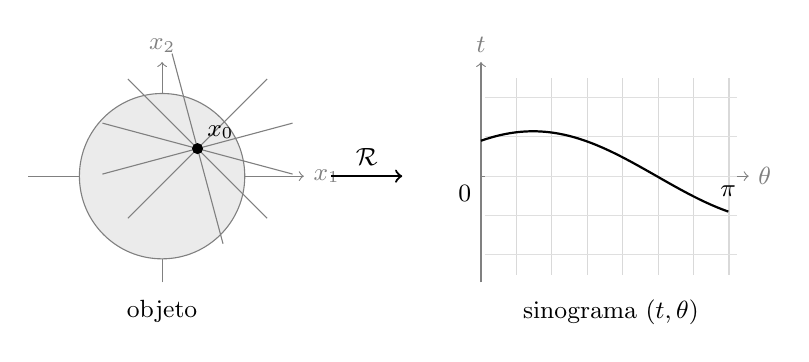
\begin{tikzpicture}[font=\small]
    \begin{scope}
        \draw[->, thin, gray] (-1.7,0) -- (1.8,0) node[right] {$x_1$};
        \draw[->, thin, gray] (0,-1.35) -- (0,1.45) node[above] {$x_2$};
        \draw[fill=black!8, draw=black!50] (0,0) circle (1.05);
        \coordinate (Xzero) at (0.45,0.35);
        \foreach \a in {15,45,75,105,135} {
            \draw[thin, gray] (Xzero) ++(\a+90:1.25) -- ++(\a-90:2.5);
        }
        \fill (Xzero) circle (2pt) node[above right] {$x_0$};
        \node[below] at (0,-1.45) {objeto};
    \end{scope}

    \draw[->, thick] (2.15,0) -- (3.05,0) node[midway, above] {$\mathcal R$};

    \begin{scope}[xshift=4.05cm]
        \draw[->, thin, gray] (0,0) -- (3.4,0) node[right] {$\theta$};
        \draw[->, thin, gray] (0,-1.35) -- (0,1.45) node[above] {$t$};
        \foreach \x in {0.45,0.9,...,3.15} {
            \draw[thin, gray!30] (\x,-1.25) -- (\x,1.25);
        }
        \foreach \y in {-1.0,-0.5,0,0.5,1.0} {
            \draw[thin, gray!25] (0.05,\y) -- (3.25,\y);
        }
        \draw[thick, black, domain=0:3.1416, samples=80, variable=\u]
            plot ({\u}, {0.45*cos(\u r)+0.35*sin(\u r)});
        \node[below left] at (0,0) {$0$};
        \node[below] at (3.14,0) {$\pi$};
        \node[align=center, below] at (1.65,-1.45) {sinograma $(t,\theta)$};
    \end{scope}
\end{tikzpicture}
\shorthandon{<>}
}
\caption{Formación esquemática del sinograma a partir de proyecciones paralelas. Elaboración propia.}
\label{fig:sinograma-diagrama}
\end{figure}

La linealidad se sigue directamente de la linealidad de la integral: para $f_1,f_2\in\mathcal S(\mathbb R^2)$ y escalares $a,b$,
\[
\mathcal R(af_1+bf_2)=a\mathcal Rf_1+b\mathcal Rf_2.
\]

Para identificar la retroproyección como adjunto formal, sea $D=\mathbb R\times(0,\pi)$. Para $u,v\in L^2(D)$ definimos el producto interno del espacio de datos por
\[
\langle u,v\rangle_{\mathrm{datos}}
=
\int_0^\pi\int_{\mathbb R}
u(t,\theta)\overline{v(t,\theta)}\,dt\,d\theta.
\]
Para $p\in L^1(\mathbb R^2)$ y $q\in L^\infty(\mathbb R^2)$ usamos la pareja de dualidad del espacio de imagen
\[
\langle p,q\rangle_{\mathrm{imagen}}
=
\int_{\mathbb R^2}p(x)\overline{q(x)}\,dx.
\]

Tomamos ahora $g\in C_c^\infty(D)$. Entonces $\mathcal Rf,g\in L^2(D)$ y $f\in L^1(\mathbb R^2)$. Definimos la retroproyección de $g$ por
\[
(\mathcal R^*g)(x)
=
\int_0^\pi
g(x\cdot\omega(\theta),\theta)\,d\theta.
\]
Además, $\mathcal R^*g\in L^\infty(\mathbb R^2)$, pues
\[
\|\mathcal R^*g\|_{L^\infty}
\leq
\pi\|g\|_{L^\infty}.
\]
Por consiguiente, en las parejas anteriores se toman concretamente $u=\mathcal Rf$, $v=g$, $p=f$ y $q=\mathcal R^*g$. Usando el cambio de variables
\[
x=t\omega(\theta)+s\omega^\perp(\theta),
\qquad dx=dt\,ds,
\]
para cada $\theta$, se obtiene
\[
\begin{aligned}
\langle\mathcal Rf,g\rangle_{\mathrm{datos}}
&=
\int_0^\pi\int_{\mathbb R}
(\mathcal Rf)(t,\theta)
\overline{g(t,\theta)}\,dt\,d\theta \\
&=
\int_{\mathbb R^2}
f(x)
\overline{
\left(
\int_0^\pi
g(x\cdot\omega(\theta),\theta)\,d\theta
\right)}\,dx \\
&=
\langle f,\mathcal R^*g\rangle_{\mathrm{imagen}}.
\end{aligned}
\]
Por tanto, la retroproyección $\mathcal R^*$ definida arriba es el adjunto formal de $\mathcal R$ con respecto a las medidas $dt\,d\theta$ y $dx$. La misma fórmula se empleará siempre que la integral angular esté bien definida. No se está afirmando aquí que ya se haya construido un operador acotado entre espacios $L^2$ completos. Para resultados de dualidad y retroproyección en un marco funcional más amplio puede consultarse Natterer \cite[Sec.~II.1, Thm.~1.3, pp.~13--15]{natterer2001}. Kuchment también desarrolla la retroproyección, aunque usa la notación $\mathcal R^\#$ y convenciones con integración angular diferentes \cite[Sec.~5.6, pp.~34--36]{kuchment2014}.

\section{Teorema de corte de Fourier}

El teorema de corte de Fourier conecta la transformada de Radon con la transformada de Fourier bidimensional. Con las convenciones del capítulo anterior, el resultado toma una forma directa.

\begin{theorem}[Teorema de corte de Fourier]
Sea $f\in\mathcal S(\mathbb R^2)$. Entonces, para todo $\theta\in[0,\pi)$ y $\sigma\in\mathbb R$,
\[
\mathcal F_t(\mathcal Rf)(\sigma,\theta)
=
\widehat f(\sigma\omega(\theta)).
\]
\end{theorem}

\begin{proof}
Usando la definición de $\mathcal Rf$ y el cambio de variables $x=t\omega(\theta)+s\omega^\perp(\theta)$, se tiene
\[
\begin{aligned}
\mathcal F_t(\mathcal Rf)(\sigma,\theta)
&=
\int_{\mathbb R}
\left(
\int_{\mathbb R}
f(t\omega(\theta)+s\omega^\perp(\theta))\,ds
\right)
e^{-2\pi i t\sigma}\,dt \\
&=
\int_{\mathbb R^2}
f(x)e^{-2\pi i\sigma x\cdot\omega(\theta)}\,dx \\
&=
\widehat f(\sigma\omega(\theta)).
\end{aligned}
\]
\end{proof}

Este resultado muestra que la transformada de Fourier unidimensional de una proyección proporciona los valores de $\widehat f$ sobre la recta radial
\[
\{\sigma\omega(\theta):\sigma\in\mathbb R\}
\]
en el dominio de frecuencias. Al variar $\theta\in[0,\pi)$, estas rectas cubren todo $\mathbb R^2$, aunque la parametrización es degenerada en el origen. El teorema de corte se encuentra, con posibles diferencias de normalización, en Helgason \cite{helgason1999}, Kuchment \cite[Sec.~5.5.4, Thm.~5.10, pp.~32--33]{kuchment2014} y Natterer \cite[Sec.~II.1, Thm.~1.1, p.~11]{natterer2001}; Kak y Slaney lo presentan en el contexto de proyecciones paralelas \cite[Sec.~3.2]{kak_slaney1988}.

\section{Fórmula de inversión}

Sea $f\in\mathcal S(\mathbb R^2)$. Partimos de la fórmula de inversión de Fourier en dos variables:
\[
f(x)=
\int_{\mathbb R^2}
\widehat f(\xi)e^{2\pi i x\cdot\xi}\,d\xi.
\]
Para reescribir esta integral en coordenadas adaptadas a la transformada de Radon, usamos el cambio con radio firmado
\[
\Phi(\sigma,\theta)=\sigma\omega(\theta),
\qquad
\sigma\in\mathbb R,
\quad
\theta\in[0,\pi).
\]
Para cada $\xi\neq0$ existe una única pareja
$(\sigma,\theta)\in(\mathbb R\setminus\{0\})\times[0,\pi)$
tal que $\xi=\sigma\omega(\theta)$. El origen es el único punto
degenerado de la parametrización y no afecta la integral.

Las derivadas del cambio son
\[
\partial_\sigma\Phi=\omega(\theta),
\qquad
\partial_\theta\Phi=\sigma\omega^\perp(\theta).
\]
Por tanto,
\[
\left|
\det\left(
\partial_\sigma\Phi,
\partial_\theta\Phi
\right)
\right|
=
|\sigma|.
\]
Así,
\[
d\xi=|\sigma|\,d\sigma\,d\theta.
\]

Sustituyendo en la inversión de Fourier y usando el teorema de corte,
\[
\begin{aligned}
f(x)
&=
\int_0^\pi\int_{\mathbb R}
\widehat f(\sigma\omega(\theta))
e^{2\pi i\sigma x\cdot\omega(\theta)}
|\sigma|\,d\sigma\,d\theta \\
&=
\int_0^\pi\int_{\mathbb R}
\mathcal F_t(\mathcal Rf)(\sigma,\theta)
|\sigma|
e^{2\pi i\sigma x\cdot\omega(\theta)}
\,d\sigma\,d\theta.
\end{aligned}
\]
Esta es la fórmula de inversión que se usará en la tesis. Con la convención de Fourier fijada y con integración angular en $[0,\pi)$, no aparece un factor adicional $1/2$ ni $1/\pi$ en esta expresión. Otras fuentes pueden usar frecuencia angular o integración sobre todas las direcciones, lo que modifica las constantes. La inversión de la transformada de Radon se desarrolla en Kuchment \cite[Sec.~5.7, pp.~36--39]{kuchment2014} y en Natterer \cite[Sec.~II.2, Thm.~2.1, pp.~18--20]{natterer2001}, con convenciones que deben convertirse antes de comparar factores.

\section{Retroproyección filtrada}

La fórmula de inversión anterior puede escribirse como un procedimiento operativo. Para cada ángulo $\theta$, se filtra la proyección $t\mapsto(\mathcal Rf)(t,\theta)$ en la variable del detector y luego se aplica la retroproyección.\\

El símbolo del filtro rampa es
\[
\tau_{\mathrm{rampa}}(\sigma)=|\sigma|.
\]
Con la notación de multiplicadores del capítulo anterior,
\[
T_{\tau_{\mathrm{rampa}}}h
=
\mathcal F_t^{-1}
\left[
|\sigma|\,\mathcal F_t h
\right].
\]
Para $f\in\mathcal S(\mathbb R^2)$, las proyecciones tienen regularidad suficiente para aplicar este multiplicador en la variable $t$.
Aplicado a cada proyección, esto produce el sinograma filtrado
\[
g_{\mathrm{filt}}(t,\theta)
=
\mathcal F_t^{-1}
\left[
|\sigma|\,\mathcal F_t(\mathcal Rf)(\sigma,\theta)
\right](t).
\]
La fórmula de inversión se convierte entonces en
\[
f
=
\mathcal R^*g_{\mathrm{filt}}
=
\mathcal R^*
\mathcal F_t^{-1}
\left[
|\sigma|\,\mathcal F_t(\mathcal Rf)
\right].
\]
Esta es la forma canónica de la retroproyección filtrada en esta tesis.
Equivalente y abreviadamente,
\[
f=\mathcal R^*T_{\tau_{\mathrm{rampa}}}\mathcal Rf,
\qquad
\tau_{\mathrm{rampa}}(\sigma)=|\sigma|.
\]

El factor $|\sigma|$ incorpora el jacobiano radial del cambio de variables, pero su crecimiento sin cota amplifica componentes de alta frecuencia. Esta observación conecta con la discusión de multiplicadores no acotados del capítulo anterior y motiva el estudio posterior de filtros modificados con símbolos $\tau(\sigma)$.

Escribiendo $g=\mathcal Rf$, la Figura~\ref{fig:fbp-flujo} presenta el procedimiento como una cadena de operaciones. Para un símbolo general $\tau$, la salida se denota $f_\tau$; para la rampa canónica $\tau(\sigma)=|\sigma|$, en el modelo continuo ideal se recupera $f$. En el capítulo computacional, la multiplicación por el símbolo se representará mediante el vector $M_\tau$, o la matriz diagonal asociada, aplicado a cada proyección en frecuencia.

\begin{figure}[htbp]
\centering
\resizebox{0.92\textwidth}{!}{\shorthandoff{<>}
\begin{tikzpicture}[node distance=1.35cm, font=\small]
    \tikzstyle{block}=[draw=black, fill=gray!10, rounded corners=2pt, minimum width=2.25cm, minimum height=0.78cm, align=center]
    \tikzstyle{data}=[align=center, minimum width=2.1cm]
    \node[data] (sino) {sinograma\\$g=\mathcal Rf$};
    \node[block, right=of sino] (fft) {Fourier en $t$\\$\mathcal F_t$};
    \node[data, right=of fft] (ghat) {$\widehat g(\sigma,\theta)$};
    \node[block, below=of ghat] (mult) {multiplicación por $\tau(\sigma)$\\(discreto: $M_\tau$)};
    \node[data, left=of mult] (gfhat) {$\widehat g_{\mathrm{filt}}$};
    \node[block, left=of gfhat] (ifft) {Fourier inversa\\$\mathcal F_t^{-1}$};
    \node[data, left=of ifft] (gf) {$g_{\mathrm{filt}}$};
    \node[block, below=of gf] (bp) {retroproyección\\$\mathcal R^*$};
    \node[data, right=of bp] (rec) {reconstrucción\\$f_\tau$};

    \draw[->, thick] (sino) -- (fft);
    \draw[->, thick] (fft) -- (ghat);
    \draw[->, thick] (ghat) -- (mult);
    \draw[->, thick] (mult) -- (gfhat);
    \draw[->, thick] (gfhat) -- (ifft);
    \draw[->, thick] (ifft) -- (gf);
    \draw[->, thick] (gf) -- (bp);
    \draw[->, thick] (bp) -- (rec);

    \node[align=center, below=0.45cm of mult]
    {rampa canónica continua: $\tau(\sigma)=|\sigma|$};
\end{tikzpicture}
\shorthandon{<>}
}
\caption{Flujo de la retroproyección filtrada en geometría paralela. Elaboración propia.}
\label{fig:fbp-flujo}
\end{figure}

La retroproyección filtrada es el algoritmo analítico clásico para datos de proyección paralela. Una presentación computacional se encuentra en Natterer \cite[Sec.~V.1, p.~102 y ss.]{natterer2001}; Kak y Slaney discuten la reconstrucción desde proyecciones paralelas en \cite[Sec.~3.3]{kak_slaney1988}. En esta tesis, la rampa se mantendrá como referencia teórica y computacional, mientras que las comparaciones numéricas posteriores reemplazarán $|\sigma|$ por otros símbolos $\tau(\sigma)$.

